% From the repository root:
% latexmk -pdf -interaction=nonstopmode -halt-on-error \
%   -outdir=/tmp/fulton-harris-plan-build docs/fulton-harris-plan.tex
% cp /tmp/fulton-harris-plan-build/fulton-harris-plan.pdf docs/
% Self-contained: no external images, bibliography, or shell escape.
\documentclass[11pt,a4paper]{article}
\usepackage[T1]{fontenc}
\usepackage{lmodern}
\usepackage[margin=23mm,headheight=15pt]{geometry}
\usepackage{amsmath,amssymb,mathtools}
\usepackage{microtype}
\usepackage[table]{xcolor}
\usepackage{booktabs,tabularx,array}
\usepackage{enumitem}
\usepackage{listings}
\usepackage{tikz}
\usetikzlibrary{arrows.meta,positioning}
\usepackage{xurl}
\usepackage{fancyhdr}
\usepackage{needspace}
\usepackage[colorlinks=true,linkcolor=teal!60!black,urlcolor=teal!60!black]{hyperref}
\definecolor{ink}{HTML}{183947}
\definecolor{muted}{HTML}{53636A}
\definecolor{pale}{HTML}{EDF4F5}
\pagestyle{fancy}
\fancyhf{}
\fancyhead[L]{\small\textcolor{ink}{Constructive Fulton--Harris in Arend}}
\fancyhead[R]{\small\textcolor{muted}{Formalization plan / 12 October 2026}}
\fancyfoot[C]{\small\thepage}
\setlength{\parindent}{0pt}
\setlength{\parskip}{5pt plus 1pt}
\setlength{\emergencystretch}{2em}
\setlist{leftmargin=*,itemsep=3pt,topsep=4pt,parsep=0pt}
\renewcommand{\arraystretch}{1.15}
\newcolumntype{P}[1]{>{\raggedright\arraybackslash}p{#1}}
\newcolumntype{Y}{>{\raggedright\arraybackslash}X}
\newcommand{\code}[1]{\texttt{\detokenize{#1}}}
\newcommand{\src}[1]{{\footnotesize\nolinkurl{#1}}}
\newcommand{\C}{\mathbb C}
\newcommand{\Q}{\mathbb Q}
\newcommand{\N}{\mathbb N}
\newcommand{\Z}{\mathbb Z}
\newcommand{\slie}{\mathfrak{sl}}
\newcommand{\g}{\mathfrak g}
\newcommand{\Hom}{\operatorname{Hom}}
\newcommand{\tr}{\operatorname{tr}}
\newcommand{\End}{\operatorname{End}}
\newcommand{\Sym}{\operatorname{Sym}}
\newcommand{\stage}[2]{\par\textbf{#1. #2}\par}
\newcommand{\decision}[1]{\begin{center}\fcolorbox{pale}{pale}{\parbox{0.94\linewidth}{#1}}\end{center}}
\lstset{basicstyle=\footnotesize\ttfamily,columns=fullflexible,keepspaces=true,
  showstringspaces=false,breaklines=true,frame=single,rulecolor=\color{pale},
  backgroundcolor=\color{pale},xleftmargin=5pt,xrightmargin=5pt,
  aboveskip=7pt,belowskip=7pt}
\hypersetup{pdftitle={Constructive Fulton--Harris in Arend: library audit and plan},
  pdfauthor={Project planning study},pdfsubject={Representation theory, arend-lib, autoformalization}}

\begin{document}
\thispagestyle{empty}
{\color{ink}\Huge Autoformalizing\\[3pt] Fulton--Harris in Arend\par}
\vspace{3mm}
{\Large A constructive variant integrated into arend-lib\par}
\vspace{3mm}
{\color{muted}Revised 12 October 2026; Maschke interface updated 20 October 2026\\
source audit: 8 October 2026\par}
\vspace{3mm}

\decision{\textbf{Integration target.} Incorporate a constructive variant directly into arend-lib.
First establish a reproducible compiler/library baseline, then complete a small
source-aligned pilot in Lectures 1--2. Extend the existing representation and
linear-algebra modules; add character theory and Lie theory in their
mathematical namespaces. Use no excluded middle or choice axioms. Replace
classical existence arguments with constructions or explicitly recorded
constructive reformulations; unresolved replacements remain research gaps.
Exercises needed for the theory receive formal statements with intentional
proof holes; dependent results retain explicit proof-status records.}

\section*{Destination and first deliverable}
The target is Fulton and Harris, \emph{Representation Theory: A First Course},
with a constructive coverage map for all 26 lectures and Appendices A--F, using
\src{\string~/Dropbox/AlgGeom/Fulton-Harris.pdf}. Exercises important for the
theory receive formal statements and named proof holes; other exercises are
deferred unless selected. Record whether each target preserves the original
statement, reformulates it, or restricts its inputs. A constructive counterpart
does not certify the unrestricted classical statement.

The first milestone covers finite-dimensional splitting and averaging, constructive
Schur variants, character identities, orthogonality for explicitly constructed
split irreducibles, and an exact $S_3$ example. A smaller pilot
precedes it: the 12 source items
on page~\pageref{sec:pilot}. This tests retrieval, statement translation,
proof repair, and semantic review before expensive Lie-theoretic work begins.

\section*{What the 8 October source audit established}
\begin{itemize}
  \item The checked-out library has 447 \code{.ard} source files, including
  representations, intertwiners, subrepresentations, averaging, Schur's lemma,
  tensors, matrices, and trace. Existing hypotheses need a constructivity audit.
  \item The representation subtree is small: nine files, approximately 450
  lines. \code{Characters.ard} is 19 lines and proves only the value at the
  identity beyond its definition and a helper. File names considerably
  overstate readiness for Lectures 1--2.
  \item Complex numbers and substantial fundamental-theorem-of-algebra
  machinery exist. The interface between constructive complex numbers and
  the discrete-field linear-algebra API requires deliberate work.
  \item No dedicated Lie-algebra, root-system, highest-weight, Young-tableau,
  or smooth-manifold development was located in the source inventory and
  targeted searches. These are substantial planned developments.
\end{itemize}

\textbf{Validation limit.} The available 1.12 executable failed on shared
\code{\Cat} syntax, then raised an exception. This audit does not certify
arend-lib. M0 must resolve the compiler pairing; see page~\pageref{sec:reproduce}.

\newpage
\section{Reusable foundations and their actual limits}\label{sec:audit}
Paths in the tables are relative to \code{arend-lib/src/}. ``Present'' means
that a definition or proof body was inspected; it does not override the
typechecking limitation on page~1. ``Gap'' means not found in the audited
interfaces and searches, and should be rechecked with the symbol index at M0.

{\small
\begin{tabularx}{\linewidth}{@{}P{28mm}YY@{}}
\toprule
Area & Present in the checkout & Remaining work for the book \\
\midrule
Representations & \code{LinRepres}, \code{TrivialAction}; actions linear over a ring. & Bundle finite dimension and distinguish abstract representations from chosen matrix presentations. \\
Maps and subobjects & \code{IntertwiningMap}, \code{KernelLRepres}, \code{ImageLRepres}; representation category and module of intertwiners. & Finite-dimensional intertwiners, invariant vectors, quotients and isomorphism-facing convenience lemmas. \\
Direct sums & \code{ProductLRepres} with inclusions, projections and a coproduct map. & Finite indexed sums, basis/dimension formulas and decomposition interfaces. Binary products model finite direct sums. \\
Schur & \code{SchurLemma}: an intertwiner between library-irreducibles is zero or an equivalence. & Replace the strong \code{IsIrreducible} definition, which implies excluded middle given a nonzero vector; adapt Schur and its callers. \\
Maschke & \code{SumOverGroup}, \code{mean_func}, \code{mean-func-preserve}. & Construct linear retractions from finite basis/independence data, then average and exhibit invariant complements. \\
Characters & \code{Character E bv g}, \code{Character.of-1}; character depends explicitly on a basis witness. & Basis independence, class functions, sums, tensors, duals, orthogonality, completeness and character tables. \\
Linear algebra & \code{FinModule}, dimension uniqueness, surjection splitting; matrix/linear-map conversion; Smith-based kernel/image finiteness. & Based/split subspaces and explicit rank computations over suitable discrete fields; separate treatment over constructive $\C$. \\
Trace and spectra & \code{Trace-prod}, \code{Trace-conjugation}, characteristic polynomial, Cayley--Hamilton. & Coordinate-free trace; trace of a projector; root-to-eigenvector bridge. \code{eigen-root} proves the opposite direction. \\
Multilinear algebra & \code{TensorProductModule}, \code{tensorLift} and uniqueness; bilinear maps; associative algebras. & Tensor bases, dual/Hom representations, tensor powers, symmetric/exterior powers, contractions and Schur functors. \\
Finite groups & Finite sets/sums, symmetric groups, cycles and signs; monoid rings. & Group-algebra representation equivalence, restriction/induction, Frobenius reciprocity, Young combinatorics and relevant finite-field examples. \\
\bottomrule
\end{tabularx}}

\textbf{Exact source anchors.} The representation definitions are under
\src{Algebra/Group/Representation.ard} and
\src{Algebra/Group/Representation/}. The intertwiner record is
\code{IntertwiningMap}, renamed from the misspelled \code{InterwiningMap}. Linear algebra is in
\src{Algebra/Module/}, \src{Algebra/Linear/VectorSpace.ard}, and
\src{Algebra/Linear/Matrix/}. Supporting constructions include
\src{Algebra/Group/Symmetric.ard}, \src{Algebra/Ring/MonoidRing.ard},
and \src{Algebra/Algebra.ard}. Preserve these names in retrieval and adapters.

\newpage
\section{Constructive foundations and statement design}\label{sec:foundations}
\stage{1}{Choice-free constructive policy}
Use Arend's type theory and justified constructive library constructions.
Exclude \code{Logic.Classical} (\code{alem}, \code{achoice}) and
\code{Logic.Choice} (\code{acchoice}, \code{adchoice}), including
transitive uses. Do not replace them with new axioms or equivalent blanket
assumptions. This plan chooses a choice-free constructive variant; finite
enumeration and proved finite-choice lemmas remain available. Audit theorem
types and definitions as well as proof bodies and meta-generated terms.

\stage{2}{Separate exact scalar computations from constructive complex numbers}
Use commutative rings for action/trace identities and an explicit inverse of
$|G|$ for averaging. Use discrete fields only where their decisions are
constructively supplied, initially $\Q$ for concrete examples. Construct
exact splitting fields, such as the needed cyclotomic extensions, with
verified operations and factorization data; their APIs are work to do.

\src{Algebra/Linear/VectorSpace.ard:43} requires \code{DiscreteField};
\src{Arith/Complex.ard:69} supplies \code{ComplexField : Field}.
Do not add decidable equality to arbitrary $\C$. Prove scalar-extension
bridges and identify precisely which results transfer. A theorem over an
exact field alone is not yet the book's theorem over constructive $\C$.
Distinguish equality, negated equality and positive invertibility/apartness
evidence whenever an algorithm divides or tests a pivot.
The explanation on page~\pageref{sec:fields-explained} makes these distinctions
concrete. Prioritize direct complex constructions and generalize library
interfaces that unnecessarily require \code{DiscreteField}; exact-field
examples supplement this work.

\stage{3}{Replace the strong irreducibility premise}
\code{IsIrreducible} quantifies over \emph{all} predicate subrepresentations.
It includes the zero representation; adding nonzeroness is insufficient.
Indeed, for any proposition $P$, the invariant submodule
\[
 W_P=\{x\mid P\lor x=0\}
\]
is allowed by \code{SubLRepres}. Given $v\ne0$, the assertion that $W_P$ is
zero or the whole space yields $\neg P$ or $P$. Thus this source definition,
with a known nonzero vector, implies excluded middle. This is a mathematical
consequence of the inspected definitions, not a newly checked Arend theorem.
Page~\pageref{sec:irreducibility-explained} gives the argument step by step
using the one-dimensional trivial representation over $\Q$.

Replace arend-lib's existing \code{IsIrreducible} definition with a reviewed
constructive formulation. M1 must settle its generality, nontriviality and
nonzero-element evidence, prove basic one-dimensional examples constructively,
and migrate Schur's lemma and its callers. The old premise must not remain
the default irreducibility interface.

\textbf{For the finite-dimensional pilot},
investigate a provisional notion testing invariant embeddings
$j:K^k\hookrightarrow V$ over a field $K$, with a chosen basis and a linear
left inverse $rj=I$ constructed from suitable finite data; $r$ need not be
equivariant. For finite-dimensional $V$ of positive
dimension, require each such embedding to have $k=0$ or be an isomorphism.
This is not the general replacement for arbitrary modules. Validate its
closure properties; for Schur's kernel/image argument, prove admissibility
using exact linear algebra where applicable. Over $\C$, prove scalar
commutants directly for constructed representations rather than assume a
zero-or-invertible test for every scalar.

\stage{4}{Keep finite data and truncated existence distinct}
\code{FinModule.isFinModule} is truncated existence of a finite basis.
Use chosen bases for computations, then prove invariance or unique existence
before eliminating truncation into a scalar or dimension. Follow
\code{FinModule.dimension-pair}; do not choose bases globally.
Supply eigenpairs/factorizations as data only for explicitly restricted
lemmas, and construct that data in concrete applications.

\newpage
\section{Why the irreducibility premise is too strong}\label{sec:irreducibility-explained}
The current definition asks too much constructively: even proving the
one-dimensional trivial representation irreducible would imply excluded
middle. The issue comes from the combination of an unrestricted notion of
submodule and the explicit assertion that each submodule is zero or everything.

\stage{The definition}{What counts as a submodule}
In \src{Algebra/Group/Representation/Irreducible.ard},
\code{IsIrreducible} says every invariant submodule is either zero or the
whole space. This looks standard. But \code{SubLRepres} allows membership
defined by \emph{any proposition}; a basis or a decision procedure for
membership is not required. Over $\Q$, these modules are vector spaces.

\stage{The example}{Encode an arbitrary proposition in a subspace}
Take $V=\Q$ with the trivial group action. Let $P$ be any proposition whose
truth we do not know, and define
\[
 W_P=\{x\in\Q\mid x=0\ \text{or}\ P\}.
\]
This is a valid invariant subspace without deciding $P$. Zero belongs to it.
For addition, if either membership proof supplies $P$, the sum belongs;
otherwise both summands are zero. Scalar multiplication also preserves
membership, and the trivial action preserves every element.

If $P$ holds, every rational number belongs to $W_P$, so $W_P=\Q$.
If $\neg P$ holds, only zero belongs, so $W_P=\{0\}$. These are conditional
statements; neither decides $P$.

\stage{The consequence}{Strong irreducibility would decide $P$}
Suppose we have proved irreducibility using the existing definition.
Applied to $W_P$, it gives $W_P=\{0\}$ or $W_P=\Q$. Either outcome settles $P$:
\begin{enumerate}
  \item \textbf{If $W_P=\{0\}$, then $\neg P$.} Otherwise $P$ would put $1$
  in $W_P$, contradicting $1\ne0$.
  \item \textbf{If $W_P=\Q$, then $P$.} Since $1\in W_P$, its membership
  means $1=0$ or $P$. The first possibility is impossible.
\end{enumerate}
Thus we obtain $P\lor\neg P$ for an arbitrary proposition $P$:
the law of excluded middle.

\stage{The proposed replacement}{A finite-dimensional pilot only}
\textbf{For the finite-dimensional pilot}, investigate irreducibility relative
to explicitly based, linearly split invariant submodules. A splitting is a
linear retraction onto the submodule that fixes its elements. This is a
provisional notion for that setting, not a universal definition of
irreducibility. We cannot generally supply the required data for $W_P$
without already settling $P$.

A finite basis restricts the submodules $W$ being tested, not logically the
ambient module $M$. Applied to an infinite-dimensional $M$, the test may miss
important infinite-dimensional invariant submodules. Over a general ring,
even a submodule of a finite free module need not be free. Keep the general
module API open to infinite-dimensional objects, including Verma modules.

The proposed notion still needs mathematical validation. For the kernel/image
proof of Schur's lemma, prove that the relevant kernels and images belong to
the permitted class.

\textbf{Replacement in arend-lib.} The existing Schur proof is valid
conditional on its old premise. Replace \code{IsIrreducible} with the reviewed
constructive definition and adapt Schur's lemma and all callers, recording
changed hypotheses or conclusions. This is a planned semantic change,
not merely a new predicate alongside the old default. The argument above
is mathematical explanation, not a newly typechecked Arend result.

\newpage
\section{What the scalar-field distinction means}\label{sec:fields-explained}
Some existing linear-algebra code assumes it can always decide whether a
number is exactly zero. Constructive complex numbers do not provide that
general zero test. This is a restriction on particular algorithms and
interfaces, not a prohibition on doing complex linear algebra.

\stage{Zero tests}{Why rational and complex numbers differ}
For a rational number, test whether its numerator is zero. For an arbitrary
constructive complex number, increasingly accurate approximations need not
settle exact equality: even knowing $|z|<10^{-100}$ does not establish $z=0$.
The number might be zero or merely very small.

These complex numbers are exact mathematical objects, not floating-point
approximations. Equality can be proved in particular cases. What is unavailable
is an assumed procedure that decides equality for every pair of complex numbers.

\stage{The library interfaces}{What the extra assumption supplies}
In \src{Algebra/Field.ard}, \code{Field} supports constructive field operations
and inversion with suitable evidence. \code{DiscreteField} additionally
provides a zero-or-invertible decision for every element, from which equality
is decidable. The current \code{VectorSpace} requires this stronger interface.
Complex vector spaces can instead use \code{LModule} over \code{ComplexField};
appropriate definitions and theorems should be generalized to that setting.

\stage{Evidence for division}{Three different assertions}
{\small
\begin{tabularx}{\linewidth}{@{}P{30mm}Y@{}}
\toprule
Assertion & What it supplies \\
\midrule
$z=0$ & A proof of exact equality. \\
$z\ne0$ & A proof that assuming $z=0$ leads to a contradiction. \\
$z\mathrel{\#}0$ (apart from zero) & Positive evidence of separation from zero, for example a rational $\varepsilon>0$ with $|z|\geq\varepsilon$, sufficient to construct an inverse. \\
\bottomrule
\end{tabularx}}
Constructively, negated equality does not automatically give this positive
evidence. In the library's \code{Field}, apartness from zero is expressed
using \code{Inv z}. A Gaussian-elimination step that divides by a pivot must
have the required evidence; it cannot silently assume an arbitrary zero test.

\stage{Scalar extension}{Allowing more scalars}
Take matrices with rational entries and let them act on $\C^n$ instead of
$\Q^n$. Matrix identities transfer, but other properties need separate proofs.
For example,
\[
 A=\begin{pmatrix}0&-1\\1&0\end{pmatrix},\qquad A^4=I.
\]
This gives a representation of the cyclic group of order four over both
fields. It has no invariant rational line: such a line would give a rational
eigenvalue $\lambda$ with $\lambda^2=-1$. Over $\C$, it splits into eigenlines
with eigenvalues $i$ and $-i$. Thus irreducibility does not automatically
transfer, even though the matrix identity does.

\textbf{Consequence for this project.} Develop complex representation theory
directly where possible, generalize unnecessarily restrictive interfaces,
and require explicit evidence where a construction needs it. Rational examples
are a useful starting point, not a replacement for the complex theory.

\newpage
\section{Constructive replacements for classical proof steps}\label{sec:replacements}
Every source item gets both an original statement and a reviewed constructive
target. Mark their relation as \code{same}, \code{reformulated}, or
\code{restricted}; use \code{research-gap} if no suitable target is settled.
A restriction is visible scope, not a proof of the unrestricted statement.

{\small
\begin{tabularx}{\linewidth}{@{}P{35mm}YY@{}}
\toprule
Book argument & Constructive deliverable & Remaining obligation \\
\midrule
Obtain basis or splitting data for an arbitrary invariant submodule & Construct an ordinary complement from finite data, then average the projection using $|G|^{-1}$. & Separate finite basis extension from obtaining bases for unrestricted predicate submodules; see below. \\
Repeatedly choose an irreducible summand & Build finite decomposition algorithms for exact, presented inputs; verify every projection and intertwiner. & Prove termination and completeness for that input class. Finite dimension alone does not decide whether a module is reducible. \\
Apply scalar Schur using an eigenvalue & Compute the commutant of constructed split irreducibles; prove it consists of scalar matrices. & A general eigenpair-relative lemma has explicit hypotheses. Prove required eigenpair data in each application. \\
Identify multiplicities and classify & Compare supplied finite decompositions using verified Hom spaces. Construct a finite family and prove exhaustiveness in the specified category. & Prove splitting-field and base-change results; never assume the desired classification as an input certificate. \\
Character inner products & Use $|G|^{-1}\sum_g\chi_V(g^{-1})\chi_W(g)$ over an exact splitting field. & Prove the complex conjugate version separately. Trace of the invariant projector gives dimension only with justified finite-rank data. \\
Choose weights and a Cartan subalgebra & Begin with explicit split Cartan/root data and finite weight decompositions; construct the classical series. & General existence and conjugacy require constructive proofs or an explicit reformulation. \\
Use compactness, integration or global geometry & Specify effective local charts, estimates, integration data and the exact conclusion needed. & Audit each analytic theorem; retain unresolved constructive replacements as research gaps. \\
\bottomrule
\end{tabularx}}

\textbf{Finite-dimensional complements.} Over a discrete field, supplied
finite bases for $W\subseteq V$ allow finite elimination or basis extension
to construct a retraction; no choice axiom is needed. Over constructive
$\C$, use positive independence evidence, such as an invertible maximal minor
of the inclusion matrix. Average the resulting retraction when $G$ is finite
and $|G|$ is invertible. The obstacle is obtaining the finite data for an
arbitrary \code{SubLRepres} from ambient finite dimension alone, as $W_P$
illustrates. Treat complement construction from those data as a reusable lemma.

\textbf{The root-selection boundary.}
\src{Arith/Complex/FTA.ard} supplies a spectrum in the completion of finite
multisets. Use this constructive output where appropriate; it is not an
individual-root selector. The inspected single-root proof in
\src{Arith/Complex/FTA/Classical.ard:155} calls \code{acchoice} and is outside
this plan. Retrieve declarations rather than stale \code{FTA.Choice} comments.
Richman's \href{https://msp.org/pjm/2000/196-1/pjm-v196-n1-p10-p.pdf}
{choice-free development of the fundamental theorem of algebra}
is the primary reference for the reformulated spectrum.

\textbf{A concrete first route.} Work out $S_3$ over $\Q$ by exact matrices.
Verify decomposition maps, scalar commutants and character pairings, then
extend the constructions to $\C$ without introducing complex equality tests.
General finite-group theory follows after explicit splitting-field and
group-algebra decomposition infrastructure. If a stronger complex statement
requires new analysis, register that bridge rather than importing choice.

\newpage
\section{The first source-aligned pilot}\label{sec:pilot}
Use Lectures 1--2 to exercise three kinds of task: a reuse wrapper, a short
new consequence, and a theorem requiring new infrastructure. The following
12 items are an initial backlog of constructive targets. Locations identify
the source inspiration; the table does not assert equivalence to every
original statement. Record each relation using page~\pageref{sec:replacements}.

{\small
\begin{tabularx}{\linewidth}{@{}P{10mm}P{31mm}YP{27mm}@{}}
\toprule
ID & Book location & Deliverable and proof approach & Dependencies \\
\midrule
P01 & \S1.1, pp.\ 3--5 & Replace \code{IsIrreducible}; define based finite representations and pilot subobjects; relate actions to $G\to\mathrm{GL}(V)$. & Constructive statement review; existing actions \\
P02 & \S1.1; Ex.\ 1.2 & Define direct sum, dual and Hom actions. State invariant Hom = intertwiners with a named exercise hole. & P01; dual/Hom basis facts \\
P03 & Schur 1.7(1), p.\ 7 & Reuse the kernel/image proof pattern with constructive admissibility evidence; package the inverse. & P01; exact kernel/image bases \\
P04 & Prop.\ 1.5, p.\ 6 & Construct a retraction from finite data, then average to obtain an invariant complement. & P01; basis/pivot data; $|G|^{-1}$ \\
P05 & Cor.\ 1.6, p.\ 6 & Compute a decomposition for the presented pilot inputs; verify maps and simplicity of summands. & P04; constructive splitting procedure \\
P06 & Schur 1.7(2), p.\ 7 & Prove scalar commutants for the constructed split irreducibles by finite matrix equations. & P01; explicit matrices \\
P07 & Prop.\ 1.8, p.\ 7 & Uniqueness of multiplicities in supplied decompositions with verified Hom dimensions. & P02, P05, P06; off-diagonal Hom vanishing \\
P08 & \S2.1, p.\ 13 & Basis-independent character, class invariance, and $\chi_V(1)=\dim V$. & P01; change of basis and trace \\
P09 & Prop.\ 2.1, p.\ 13 & First establish sum, tensor and dual character formulas; leave the exterior-square conjunct explicitly pending. & P02, P08; tensor bases \\
P10 & Ex.\ 2.5, p.\ 14 & State the permutation-character fixed-point formula; leave its proof as a named exercise hole. & P08; \code{PermRepr}; finite sums \\
P11 & Prop.\ 2.8, p.\ 15 & Average onto invariants; relate trace to dimension when the image has certified finite-rank data. & P08; idempotent trace; exact rank \\
P12 & Thm.\ 2.12, p.\ 16 & Orthogonality for the constructed split irreducibles, using the inverse-character pairing. & P02, P06, P09, P11; Hom vanishing \\
\bottomrule
\end{tabularx}}

\textbf{Order.} Begin P01, P04 and P08; register P02/P10 exercise holes.
Validate the admissibility API with P03 and the $S_3$ constructions before
generalizing P05--P07. P09 remains partial until the exterior-square formula
is included. Prove that the inverse-character pairing specializes to the
book's conjugate pairing when making that comparison.

\textbf{A concrete regression example.} Construct the trivial, sign and
two-dimensional standard representations of $S_3$ over $\Q$. Prove that the permutation
representation on three letters splits as $1\oplus V_{\mathrm{std}}$ and derive
the character rows $(1,1,1)$, $(1,-1,1)$ and $(2,0,-1)$ on the identity,
transposition and three-cycle classes. Verify the class sizes $1,3,2$ and
orthogonality by exact arithmetic. Then prove base change to $\C$.
Exhaustiveness requires its own constructive completeness proof.

\textbf{Pilot exit.} Review every statement. Check non-exercise proofs where
dependencies permit; retain P02's exercise component and P10 as holes.
Report downstream results that depend on these holes as conditional or pending,
including any affected $S_3$ checks. Exercise holes are not proof-search tasks.

\newpage
\section{Theory exercises remain explicit holes}\label{sec:exercises}
An exercise is important for the theory when later definitions or arguments
use its result, or when it supplies a construction needed by the chosen proof
route. Record that role and the consuming declarations. Formalize its full
statement in the appropriate arend-lib mathematical module, with explicit
hypotheses and an intentionally unfinished proof body. Review its constructive
formulation before registering the hole. The autoformalizer
must leave that body open rather than solve the exercise.

\textbf{Representation.} Use an Arend goal expression such as
\code{{?FH_L01_Ex1_2}} as the proof body. Give it a stable source identifier,
cite the exercise in the declaration's doc comment, and list it in the
coverage manifest. The hole is part of the planned deliverable, not a missing
task to be retried. Do not replace it with an axiom, insert a solution under
a helper name, or silently discharge it by applying an existing theorem.
An exercise hole must not conceal excluded middle, choice, or an unreviewed
classical existence principle. Record any reformulation in its source entry.

\textbf{Immediate examples.} Exercise 1.2 identifies the invariant vectors
in $\Hom(V,W)$ with intertwiners. P02 builds the representation constructions,
but leaves this identification as an exercise hole. Exercise 2.5 gives the
fixed-point formula for permutation characters; P10 is a statement and hole,
not a request to prove that formula. These results are used in the character
theory, so their downstream dependencies remain visible.

\begin{lstlisting}
id: FH.L01.Ex1.2
kind: exercise
theory_role: "Identifies invariant Hom with intertwiners"
formal_target: Algebra.Group.Representation.Hom:invariantHom
status: intentional-exercise-hole
statement_review: required
source_relation: same  # confirm during constructive statement review
proof_policy: leave-hole
goal_name: FH_L01_Ex1_2
consumers: [FH.L02.Thm2.12]
\end{lstlisting}
The declaration name is proposed; the source identifier remains stable even
if the mathematical API changes. The consumers list is populated from the
actual proof route, including transitive dependencies in generated reports.

\textbf{Downstream development.} Continue writing later theory against the
reviewed exercise statement where Arend permits it, while recording the
dependency on its hole. Such a result is not an unconditional checked proof.
If the checker cannot elaborate a consumer of an open declaration, keep it
pending, or check a clearly conditional helper with the exercise statement
as an explicit parameter. Neither approach closes the original exercise hole.

\textbf{Validation.} Check signatures and all available proof bodies. Match
intentional exercise goals to the manifest by declaration, location and goal
name. Distinguish their expected diagnostics from unexpected type errors,
unregistered holes and remaining downstream obligations. A run containing
expected goals is a development report, not a clean proof certification.
The subset reported as fully verified must have no holes in its dependency
closure. M0 must establish how the pinned checker reports goals and consumers.

\textbf{Completion policy.} A theory milestone may be complete with the
registered exercise statements left open. Report proved assertions,
intentional exercise holes, conditional/pending consumers and deferred items
separately. Non-exercise gaps still require proofs or explicit pending status.
Leave exercises outside the theoretical dependency graph deferred unless
selected; their solutions are not part of the automatic proof backlog.

\newpage
\section{Whole-book coverage map}\label{sec:coverage}
Fulton--Harris is organized pedagogically. Implementation should follow
dependencies, especially the appendices used by later lectures. This table
accounts for the full destination. All targets below mean constructive
variants subject to page~\pageref{sec:replacements}; general existence and
analytic results require statement-level feasibility review.

{\small
\begin{tabularx}{\linewidth}{@{}P{27mm}P{43mm}Y@{}}
\toprule
Book unit & Target & Development needed \\
\midrule
Lectures 1--2 & Finite representations and characters & Pilot; explicit splitting fields and group-algebra matrix blocks; constructive completeness, multiplicities and isotypic projectors. \\
Lecture 3 & Induction, group algebras, real representations & Finite coset data, induction, Frobenius reciprocity, $K[G]$-module equivalence, exterior powers and certified real/complex descent. \\
Lectures 4--6 & Symmetric/alternating groups, finite $\mathrm{GL}_2$, Weyl's construction & Partitions, tableaux, Young symmetrizers, symmetric functions, Frobenius character formula and Schur functors; finite-field and alternating-group branches. \\
Lectures 7--8 & Lie groups, Lie algebras, exponential & Algebraic brackets first; constructively specified manifolds, tangent spaces and exponential maps form a separate research track. \\
Lectures 9--10 & Structure and low dimensions & Explicit ideals, nilpotence/solvability witnesses; constructive Engel/Lie variants and radicals. Audit eigenvector and subspace choices. \\
Lectures 11--13 & $\slie_2$, $\slie_3$, plethysm & Explicit raising/lowering operators and polynomial modules; classification initially for supplied finite weight decompositions. \\
Lecture 14 & Semisimple structure & Killing form, explicit split Cartan data, roots/weights and highest weights; general existence is a separate obligation. \\
Lectures 15--19 & Classical series & $\slie_n$, symplectic and orthogonal Lie algebras; root data, dominant weights and tensor constructions, including low-rank coincidences. \\
Lecture 20 & Spin & Clifford algebras, spin modules and triality; Lie-group realization depends on the analytic track. \\
Lectures 21--22 & Classification and exceptional types & Finite root data, Dynkin algorithms, explicit reconstruction and exceptional modules. State which supplied structures are classified. \\
Lectures 23--25 & Groups and character formulas & Weight lattices, representation rings, Weyl/Freudenthal/Kostant formulas, branching; homogeneous spaces and Bruhat geometry are explicit additional obligations. \\
Lecture 26 & Real forms and representations & Explicit conjugations and real/quaternionic structures; constructive compact-group theory remains a research dependency. Track both character-formula routes. \\
Appendices A--B & Symmetric functions; multilinear algebra & Move tensors, duals, exterior/symmetric powers and symmetric-function identities before their first use in Lectures 2--6. \\
Appendices C--D & Semisimplicity; Cartan subalgebras & Constructive Cartan criterion, splitting, Jordan data and Weyl groups; audit Cartan existence/conjugacy before admitting statements. \\
Appendices E--F & Levi/Ado; invariant theory & Explicit enveloping-algebra constructions; constructive Levi/Ado variants, invariants and Capelli identity. Register unresolved replacements. \\
\bottomrule
\end{tabularx}}

\textbf{Coverage discipline.} Report source relation and proof status on
separate axes. A proved restricted variant, an open generalization and a
reviewed exercise hole are three different deliverables.

\newpage
\section{How to build the missing Lie theory}
\stage{Algebraic interfaces}{Small reusable structures}
Define a Lie algebra over a commutative ring as a module with a bilinear,
alternating bracket and Jacobi identity. Define homomorphisms, ideals,
subalgebras, quotients, the adjoint action and Lie modules. Prove that
commutators in an associative algebra give a Lie algebra. Build $\mathfrak{gl}(V)$
and $\slie(V)$ using endomorphisms and trace, with matrix models for calculations.
Keep the zero bracket and characteristic-sensitive cases in view.

\stage{First independent milestone}{$\slie_2$ and explicit representations}
Prove the relations
\[
 [h,e]=2e,\qquad [h,f]=-2f,\qquad [e,f]=h.
\]
Construct $\Sym^n(K^2)$ with explicit bases and coefficient formulas.
Prove simplicity for the selected admissible-submodule notion and specify
the inverses of positive integers used in characteristic zero. Construct
Clebsch--Gordan maps and their inverses. First classify modules carrying an
explicit finite weight decomposition and suitable highest-weight data;
do not silently assume every module comes with these witnesses.
Proving their existence for a broader class is a separate task. This
milestone validates the Lie APIs before general classification.

\stage{Structural results}{Move prerequisites before users}
Audit Engel/Lie, Cartan's criterion, Jordan decomposition and semisimple
splitting for uses of eigenvectors, maximal subspaces and nonconstructive
case splits. Start with explicit split Cartan subalgebras and root-space
data, then seek constructive existence and conjugacy results corresponding
to Appendices C--D. Define finite root systems independently and implement
Dynkin classification with checked certificates. Prove the bridge to Lie
algebras: classifying root data alone does not classify all complex Lie algebras.

For general highest weights, plan explicit universal-enveloping-algebra,
PBW and highest-weight-module infrastructure if that proof route is selected.
Keep the Lie-module interface unrestricted in dimension so it can accommodate
Verma modules; the finite-dimensional pilot's submodule criterion is local
to that pilot.
Use explicit ordered monomials and reductions. After the $\slie_2$ pilot,
audit existence proofs for choices of maximal submodules. If an alternative
construction follows the book more directly, record that proof route and its
dependencies instead. No temporary ``highest-weight theorem'' axiom counts
toward completed results.

\stage{Character formulas}{A proof, not only a formula evaluator}
Represent formal characters in the group ring of a weight lattice, reusing
monoid-ring machinery where appropriate. Develop Weyl-group actions,
positive roots, the denominator identity and the representation-theoretic
argument needed for the Weyl character formula. Separate a verified
combinatorial algorithm for weights from the theorem identifying its output
with the character of a module. Then derive dimension, multiplicity, tensor
product and restriction formulas and test low ranks against explicit modules.

\stage{Lie groups and geometry}{A constructive research track}
The library contains topology, analysis and a synthetic derivative interface,
but no ready-made manifold/Lie-group package was found. Audit the real and
complex differentiable setting before choosing an implementation. Specify
the data and estimates needed for inverse-function/exponential results,
coverings, integration of Lie-algebra maps and compact-group averaging.
Finite-group averaging does not supply Haar integration. Treat global
existence theorems as research gaps until a constructive formulation and proof
route are reviewed. Develop homogeneous/flag spaces and Bruhat arguments
under explicit hypotheses. Record any algebraic replacement and its relation
to the source; omitted geometry remains visible in coverage.

\newpage
\section{The autoformalization workflow}\label{sec:pipeline}
Automate one dependency-ready assertion at a time. The controller must
separate source interpretation, declaration design, proof generation and
acceptance. First classify theory exercises as intentional holes
(page~\pageref{sec:exercises}). A typecheck verifies a formal statement,
not its fidelity to the book.

\begin{enumerate}
  \item \textbf{Extract and align.} Use the PDF text layer for search and page
  images for formulas. The text extraction visibly confuses $S_d$, $A_d$,
  $\slie_n$, $\oplus$, superscripts and theorem numbers (e.g.\ 2.8).
  Store both printed page and physical PDF page; validate each mapping rather
  than assume one constant offset throughout the scan.
  \item \textbf{Normalize the claim.} Create a short mathematical statement,
  explicit hypotheses, notation bindings and a proposed Arend declaration.
  Split multi-part propositions. Resolve phrases such as ``canonical'',
  ``unique'' and ``by Schur'' into separate obligations. Review the statement
  before broad proof search. Review constructivity: record a same-statement
  translation, a reformulation or an input restriction. Specify the data
  replacing each classical choice. Unsettled replacements are research gaps.
  \item \textbf{Retrieve exact dependencies.} Search definitions by name,
  signature shape, class hierarchy and usages. Supply the generator with
  actual declarations, hypotheses, import paths and nearby proof patterns.
  Filter by the constructive dependency policy; classical lemmas and the
  strong \code{IsIrreducible} premise are not default proof templates.
  \item \textbf{Plan a proof and register gaps.} Prefer an application of an
  existing theorem, then a short composition of lemmas, then new foundation
  work. Register an exercise dependency as a named intentional hole and track
  its consumers. For other missing lemmas, create proof tasks and postpone
  consumers. Never insert a result as an untracked assumption.
  \item \textbf{Generate, elaborate, repair.} Work in an isolated working copy
  of the target arend-lib module. Try local proof steps using \code{rewrite}, \code{exts},
  \code{equation}, \code{linarith}, \code{cases} and \code{simplify} metas where
  their domains apply. Feed exact diagnostics and relevant goals back into a
  bounded repair loop; save unsuccessful attempts. Exclude intentional
  exercise holes from generation and repair.
  \item \textbf{Review and certify.} Check source fidelity, quantifiers,
  nonzeroness, characteristic, finiteness, equality versus isomorphism and all
  additional hypotheses and constructive source relation. Inspect the elaborated result, then perform a fresh
  typecheck with secondary checking. A fully verified result has no holes in
  its dependency closure. Report intentional exercise goals and their consumers
  separately; reject unregistered gaps, forbidden axioms and hidden classical
  strength in hypotheses. A parameterized classical principle is still outside
  the constructive target.
  \item \textbf{Integrate a small accepted increment.} Add the proof to its
  arend-lib mathematical module, with provenance and regression examples.
  Check affected consumers and library tests. Add a reusable proof pattern to
  retrieval only after review. Integrate registered exercise holes as statements,
  preserving their status and downstream dependencies in coverage reports.
\end{enumerate}

\textbf{Use the tools already in this checkout.} The CLI exposes
\code{-ss} for names, \code{-ps} for signature-shape retrieval,
\code{-fu} for usages, \code{-ch} for hierarchy and \code{-sc} for scope.
The retrieval commands support \code{--json}; \code{-p} prints elaborated
definitions after checking. In particular, \code{-ps} is retrieval of existing
declarations, not a general automatic proof synthesizer. Verify these
capabilities against the newly pinned executable before relying on them.

\textbf{Stopping rule.} Start with a modest fixed per-assertion retry/token
budget, for example five repair cycles. Classify exhaustion as source
ambiguity, missing library lemma, elaboration failure or proof-search failure.
Do not repeat essentially identical attempts or silently weaken the theorem.
Revisit the task once the missing dependency or interface issue is resolved.

\newpage
\section{Integration into arend-lib and evidence records}
Use arend-lib's existing \code{arend.yaml}, source tree and test suite.
Definitions and theorems belong in mathematical namespaces; book numbers
belong in documentation and provenance records. The layout below proposes
extensions to arend-lib. This planning task updates only the TeX and PDF in
the repository's \code{docs/} directory.

\begin{lstlisting}
arend-lib/
  arend.yaml                         # existing library configuration
  src/
    Algebra/Group/Representation/    # extend Schur, Maschke, characters
    Algebra/Module/                  # duals, tensors, exterior/symmetric powers
    Algebra/Linear/                  # finite bases, rank, split subspaces
    Algebra/Group/Symmetric/         # representation theory of symmetric groups
    Combinatorics/                   # partitions and tableaux
    Algebra/Lie.ard, Algebra/Lie/    # new Lie algebra/module/root/weight APIs
    Topology/, Analysis/, AG/        # group/geometry foundations as needed
    Arith/Complex/                   # constructive spectra and base change
  test/Algebra/                     # exact examples and API regressions
  docs/fulton-harris/                # source manifest, dependencies, coverage
  tools/autoformalization/           # retrieval, generation/checking controller
\end{lstlisting}

\textbf{A source record.} Use a machine-readable schema such as JSON Lines.
For the finite-dimensional constructive Maschke variant, record at least:
\begin{lstlisting}
id: FH.L01.Prop1.5
kind: proposition
source: {printed_page: 6, pdf_page: 21, label: "Proposition 1.5"}
original: "Every invariant subspace has an invariant complement."
constructive: "Build and average a retraction for a based invariant subspace."
source_relation: restricted
data: [finite_group, inverse_of_group_order, based_inclusion]
linear_algebra: discrete_field_or_certified_pivots
formal_target: Algebra.Group.Representation.MaschkeLemma:finiteDimComplement
dependencies: [GAP.finiteDimRetraction, mean-func-preserve]
status: planned
statement_review: pending
proof_check: not_run
axiom_policy: no_excluded_middle_or_choice
axiom_audit: pending
\end{lstlisting}
The target name above is a design placeholder, not an existing theorem.
Once checked, add the exact compiler/library/source hashes, declaration
signature hash, import/declaration dependencies, command, exit status, log
location, proof route, axiom dependencies and reviewer outcome.

\textbf{States.} Use \code{extracted}, \code{statement-reviewed},
\code{blocked-on-dependency}, \code{candidate}, \code{checked}, and
\code{accepted}; permit an explicit \code{deferred} state. ``Checked'' and
``accepted'' are separate. Add \code{intentional-exercise-hole} and
\code{conditional-on-exercises}; neither means fully proved. Reused results
map to library declarations after statement review. Keep exercise holes open.

\textbf{Dependency graph.} Maintain both the source-level mathematical DAG
and the actual declaration/import graph, including types and definitions.
Use them for work order, rechecking and axiom provenance. Track a missing lemma as
a named node with intended signature, consumers and acceptance condition.
If elaborated dependency export is insufficient, start with a conservative
import audit and label its limitation rather than claim exact axiom usage.

\textbf{Library maintenance.} Replace \code{IsIrreducible} and migrate its
theorems and callers in a checked change, documenting semantic differences.
Extend mathematical modules directly in arend-lib with affected-consumer
checks and tests under \code{arend-lib/test/}. Use mathematical names and
source provenance. Exclude classical dependencies from accepted results.

\newpage
\section{Milestones, dependencies and stopping gates}\label{sec:milestones}
These are acceptance milestones, not elapsed-time promises. Later stages have
more uncertainty than the finite-group pilot. Each stage incorporates its
mathematics and tests into arend-lib under the constructive policy. Registered
exercise holes satisfy the statement deliverable; their consumers remain
conditional/pending. Research gaps prevent claims of full theory completion.

{\small
\begin{tabularx}{\linewidth}{@{}P{10mm}P{28mm}YP{27mm}@{}}
\toprule
Stage & Deliverable & Exit evidence & Needs \\
\midrule
M0 & Reproducible baseline & Pin compiler/extensions; check required modules; establish goal and axiom reporting; reject an invalid-proof control. & None \\
M1 & Constructive interfaces & Replace \code{IsIrreducible} and migrate callers; validate constructive examples and pilot interfaces; check P01/P03/P04/P08 and register P02/P10 holes. & M0 \\
M2 & Finite-group core & Exact $S_3$, pilot and Prop.\ 2.1 variants; construct splitting fields and completeness for specified inputs. Verify bridges to $\C$; retain exercise holes. & M1; linear and multilinear bridges \\
M3 & Remaining Part I & Constructive Lectures 3--6 and A--B: induction, Young theory, Schur functors and finite-field examples; record source relations. & M2 \\
M4 & Algebraic Lie pilot & Lie APIs; explicit $\slie_2$ modules and Clebsch--Gordan; classification for reviewed weight-decomposed inputs. & M1; relevant B material \\
M5 & Split Lie structure & Split Cartan/root data, highest weights; constructive Engel/Lie and C--D variants. General existence gaps tracked separately. & M4; C--D; M3 tensor tools \\
M6 & Advanced algebra & Explicit classical/exceptional series, spin, Dynkin reconstruction and character formulas; reviewed E--F variants. & M3, M5 \\
M7 & Groups and geometry & Constructive analytic foundations and reviewed group/geometry variants. Unresolved replacements remain research gaps. & M0; analytic audit; M4--M6 as needed \\
M8 & Coverage reconciliation & Every source item mapped to its constructive target or gap; fresh proof/axiom audit; holes and consumers reported. Full completion requires all agreed gaps closed. & M2--M7 \\
\bottomrule
\end{tabularx}}

\begin{center}
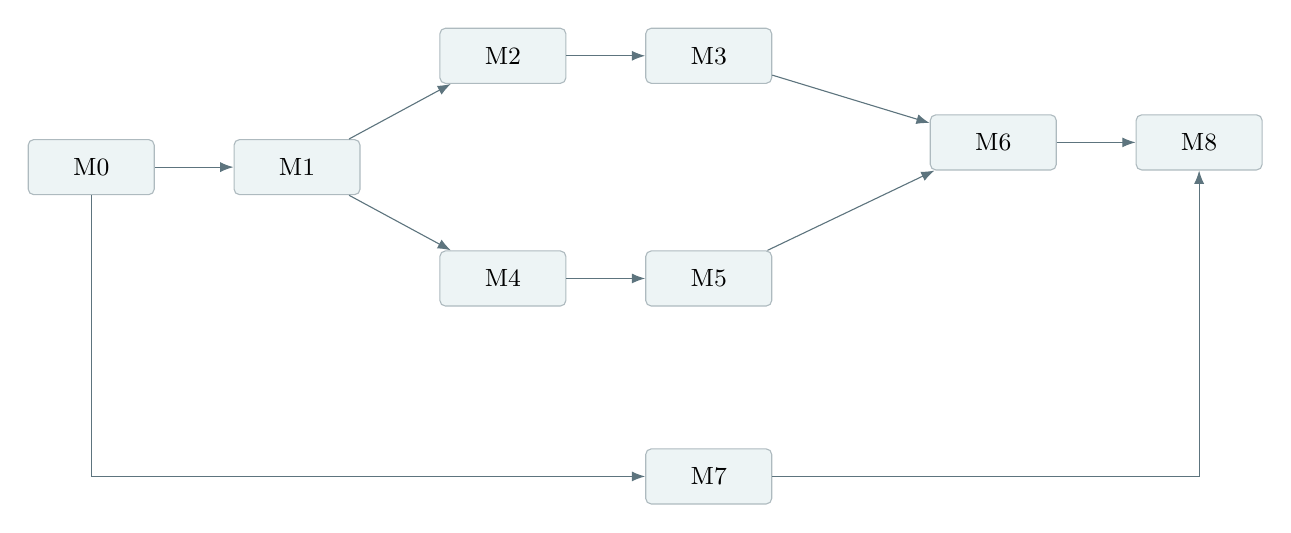
\begin{tikzpicture}[>=Latex,node distance=7mm and 10mm,
  box/.style={draw=ink!35,fill=pale,rounded corners=2pt,minimum height=7mm,
    minimum width=16mm,font=\small},every path/.style={draw=ink!70}]
\node[box] (m0) {M0};
\node[box,right=of m0] (m1) {M1};
\node[box,above right=of m1] (m2) {M2};
\node[box,right=of m2] (m3) {M3};
\node[box,below right=of m1] (m4) {M4};
\node[box,right=of m4] (m5) {M5};
\node[box,right=20mm of m3,yshift=-11mm] (m6) {M6};
\node[box,below=18mm of m5] (m7) {M7};
\node[box,right=of m6] (m8) {M8};
\draw[->] (m0)--(m1);
\draw[->] (m1)--(m2); \draw[->] (m2)--(m3);
\draw[->] (m1)--(m4); \draw[->] (m4)--(m5);
\draw[->] (m3)--(m6); \draw[->] (m5)--(m6); \draw[->] (m6)--(m8);
\draw[->] (m0.south) |- (m7.west);
\draw[->] (m7.east) -| (m8.south);
\end{tikzpicture}
\end{center}
{\small The diagram shows major work streams; the table retains cross-dependencies.
M4 need not wait for all symmetric-group and finite-field material. M7 can
begin its foundation audit early and joins the final completion gate.}

\newpage
\section{Quality, effort measurement and project risks}
\stage{Acceptance}{Distinguish proved results from exercise holes}
\begin{enumerate}
  \item \textbf{Semantic review:} the mathematical assertion and formal
  signature agree in quantifiers, hypotheses and exceptional cases. Record
  the original and constructive statements and their relation. A reviewed
  restriction is a valid variant; the stronger source claim remains separate.
  Do not add hypotheses merely to make proof search succeed.
  \item \textbf{Proof review:} check the declaration and dependency closure
  from source with no goals, placeholders, excluded middle or choice axioms.
  Confirm the expected modules were processed. Exercise holes receive
  statement review; their consumers remain conditional/pending.
\end{enumerate}
Test rejection of an invalid proof of $0=1$ in $\N$ and detection of a
choice-dependent declaration. Record the trusted compiler, prelude and
extensions. These are harness checks, not consistency tests.

\textbf{Regression cases.} Check zero/trivial representations, basis changes,
$S_3$, and characteristic $p\mid |G|$, where Maschke's inverse is unavailable.
Later add $\slie_2$ weights and low-rank characters. Check that simplicity
avoids arbitrary proposition-submodule dichotomies and complex base change
requires no equality oracle.

\stage{Measurement}{Estimate after the pilot}
Calibrate over roughly ten working days: M0, M1 statements/proofs and one
substantive bridge. If M0 consumes this timebox, reschedule the proof pilot.
Report source relations, proof statuses, exercise holes, blocked dependencies,
reuse, attempts, human review time, generation cost and checking time.
Separate wrappers, routine algebra, bridges and major theorems.

Estimate remaining work per task class using observed median and
upper-quartile effort, with separate uncertainty ranges for untested Lie and
geometry foundations. This audit supports no automation-success rate or
completion date. Budget exercise statements, excluding solutions to their
intentional holes. Helper-lemma counts are not book-theorem counts.

{\small
\begin{tabularx}{\linewidth}{@{}P{36mm}YY@{}}
\toprule
Risk & Early signal & Response \\
\midrule
Compiler/library mismatch & Parse failures before the target proof & Rebuild and pin at M0; record source and executable hashes. \\
Wrong formal statement & Proof succeeds only after adding assumptions & Freeze reviewed signatures; return to dependency planning. \\
Field/basis mismatch & Implicit-instance failures or illegal extraction of a basis & Use explicit adapters and basis-independence lemmas. \\
Hidden classical strength & A lemma needs arbitrary zero tests or unrestricted subobject dichotomies & Audit hypotheses, not just axiom names; revise the target explicitly. \\
Hidden analytic dependency & A Lie-algebra argument invokes compact groups or geometry & Route to M7, or supply a proved algebraic replacement and record it. \\
Proof-search stagnation & Repeated failures with the same missing fact & Stop retries; create a reusable lemma task. \\
Overstated coverage & Exercise holes or their consumers counted as proved & Report proof status, intentional holes and deferred items separately. \\
\bottomrule
\end{tabularx}}

\newpage
\section{Reproducibility and source notes}\label{sec:reproduce}
\textbf{Audit provenance.} The constructive revision is dated 12 October
2026. Relevant irreducibility, submodule and FTA definitions were reread for
this revision. Inventory counts and the compiler experiment below are from
8 October; the compiler experiment was not rerun. The audited Git revision was
\src{17fe0520676cefeb38a9fcb3568f94c0ef9028fb} (30 September 2026,
``Fix serialization''). \code{arend-lib/} is tracked in this same repository,
not a separate submodule. Its \code{arend.yaml} declares language/library
version 1.12, \code{src}, \code{test}, \code{bin}, and the extension entry point
\code{org.arend.lib.StdExtension}. Existing untracked \code{docs/} material
was present before this planning task.

\textbf{Book identity.} The supplied PDF has 559 physical pages and a searchable
text layer. SHA-256:
\src{83a1d9cb639aa8c548de87682dc4f4a799dfde06c8f46977a386a524c1e3eeb1}.
The contents pages and selected early theorem pages were visually inspected.
The study read the early representation/character statements and audited
relevant library bodies; it did not verify every proof in all 26 lectures.
The later roadmap is a dependency assessment from the book's structure and
the source inventory, not a completed theorem-by-theorem extraction.

\textbf{Baseline experiment.} Java reported OpenJDK 21.0.10. The available
\code{cli-1.12.0-full.jar}, dated 19 September 2026, had SHA-256
\src{ba31ff5c574b0d79b76163b62c5fc871493027f87db452c0cd9c913a2fa1be1f}.
From the repository root, this command exited with status 1:
\begin{lstlisting}
java -Xmx4g -jar cli/build/libs/cli-1.12.0-full.jar arend-lib \
  Algebra.Group.Representation.Irreducible \
  Algebra.Group.Representation.MaschkeLemma \
  Algebra.Group.Representation.Characters -r -c
\end{lstlisting}
It failed while processing shared dependencies: the first reported error was
\code{Equiv:15:24}, rejecting \code{\Cat}; further parser errors preceded
\code{IndexOutOfBoundsException} in name resolution. This is evidence that
the available executable/source pairing is unsuitable, not evidence that
Schur's lemma or Maschke's mathematics is false. No library proof was counted
as freshly verified by this experiment.

\textbf{Proposed M0 commands; not executed as part of the plan.}
\begin{lstlisting}
./gradlew :cli:jarDep :arend-lib:meta:classes
# Verify the rebuilt executable's help, version and hashes, then:
java -Xmx4g -jar cli/build/libs/cli-1.12.0-full.jar arend-lib -r -c
java -Xmx4g -jar cli/build/libs/cli-1.12.0-full.jar arend-lib -t -r -c
# During the pilot, check the affected arend-lib modules, for example:
java -Xmx4g -jar cli/build/libs/cli-1.12.0-full.jar \
  arend-lib Algebra.Group.Representation.Irreducible -r -c
\end{lstlisting}
Use a clean process and no stale binary caches for acceptance. If the rebuilt
CLI can route to an existing daemon, use its documented \code{--no-daemon}
option so fresh-check flags take effect. Do not assume options in current
source documentation are implemented by an older bundled JAR.

\textbf{Primary references.} The local source files named throughout this
document are the evidence for the audit. Operational references are
\src{ARCHITECTURE.md}, \src{settings.gradle.kts},
\src{arend-lib/meta/build.gradle.kts}, and
\src{cli/src/main/java/org/arend/frontend/doc/ConsoleMain-arguments.md}.
Meta implementations are registered in
\src{arend-lib/meta/src/main/java/org/arend/lib/StdExtension.java}.
The \href{https://arend-lang.github.io/documentation/}{official Arend documentation}
and \href{https://github.com/JetBrains/arend-lib}{upstream arend-lib repository}
were consulted on 8 October 2026 for orientation; availability claims here
refer to the local snapshot, which may differ from upstream.

\end{document}
